\documentclass[a4paper]{article}
\usepackage[english]{babel}
\usepackage[utf8]{inputenc}
\usepackage{alltt,amsmath,hyperref,graphicx}
\usepackage[usenames,dvipsnames]{xcolor}

% Link colors
\hypersetup{colorlinks=true,linkcolor=black,urlcolor=blue,citecolor=OliveGreen}

% Set paragraph indentation
\parindent 0pt
\parskip 1.0ex plus 0.5ex minus 0.2ex

\title{Internet Programming - Assignment 1}
\author{Jayke Meijer, 2526284, jmr251, \url{jayke.meijer@gmail.com}}

\begin{document}

\maketitle

\tableofcontents
\pagebreak

\section{Used platform}



\section{Writing a Micro-Shell}

The first exercise of assignment 1 is to write a number of shell programs and to answer
some questions about them.

\subsection{mysh1}

The first shell reads a command and executes it. The command does not yet have arguments.
To be able to do this, once the command is read and verified, the process forks. The child
process than proceeds to execute the command using \texttt{execlp()}. The parent waits for
the child to complete, than asks for a new command.

\subsection{mysh2}

Mysh2 is an extension of the first shell. It is capable of handling execution of programs
with arguments. The command string is split on spaces. Each of the arguments is put in an
array, and the execution is started using \texttt{execvp()}, which has the ability to pass
a NULL-terminated array to the executed program as ``commandline''-arguments.

\subsection{mysh3}

The third shell supports a piped operation. Two processes are started, and the output of
the first is the input of the second. For example, the command \texttt{ls /tmp | wc -l} 
has to be possible.

This means the command has to be split first. If no pipe is required, execution is like in
mysh2. Otherwise, there are two design possibilities. The parent has to fork a child that 
will start the first process. That child can than fork the second child process, that
will execute the second program. The other option is that the second child is spawned by
the initial parent process. See also figure \ref{tree}.

\begin{figure}
    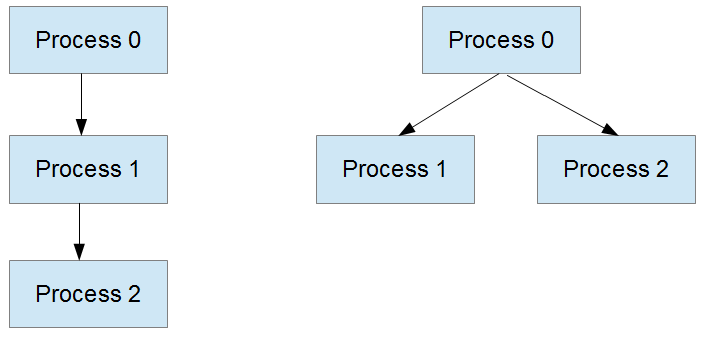
\includegraphics[scale=.5]{img/tree.png}
    \caption{The two design options. Process 0 can spawn just process 1, which in turn 
        spawns process 2, or process 0 can spawn both child processes.}
    \label{tree}
\end{figure}

The second option is used in this program. This allows the parent to create the second
process while the first is initializing itself. It also is more true to what seems to 
happen, the parent `owns' both programs, the first child does not own the second.

\subsection{Answers to the questions}

\begin{itemize}
    \item \textbf{Question A} The process must create three processes: The parent, the 
            first child program and the second child program. One pipe has to be created,
            because there only has to be one-directional communication: the output of the
            first process to the input of the second. The shell has to wait until both
            child processes are finished before being able to accept another command.
    \item \textbf{Question B} You can not implement a shell program that uses threads
            instead of processes. To be able to execute a new process, the \texttt{exec}
            call has to be used. This call takes over the entire process. Since threads
            are all part of the same process, this will end all threads of the shell 
            program, effectively killing the shell.
    \item \textbf{Question C} No, this is not possible. \texttt{cd} is part of the 
            original shell and changes value there. Since a child cannot alter the state
            of its parent, \texttt{cd} is not possible in the shell that was written for 
            this assignment.
\end{itemize}

\end{document}